\documentclass{beamer}
\usepackage{etex}

\usepackage[utf8]{inputenc}
\usepackage[T1]{fontenc}

\usepackage[french]{babel}

\usepackage{amsmath} 
\usepackage{graphicx}
%\usepackage{wrapfig}
\usepackage{amsmath}
\usepackage{array}
\usepackage{amsfonts}
%\usepackage{mathtools}
\usepackage{amssymb}
\usepackage{bbm}
\usepackage{pdfpages} %inclusion de fichier pdf!
%\usepackage[left,pagewise]{lineno}  
%\usepackage{float}   %pour forcer les figuester ou elles sont !! 
\usepackage{multibib} %bibliomultiple  cf doc "multibib" sur le net
\usepackage[normalem]{ulem} %barrer un mot
\usepackage{fancyvrb}
\usepackage{listings, multicol, xcolor} % Listings
\usepackage{lmodern}
\usepackage{url, hyperref} % Urls

%pour colorer du \verb nom \colorverb
\usepackage{xcolor}



% \meta command, a la doc
\newcommand{\meta}[1]{\ensuremath\langle\itshape#1\ensuremath\rangle}

\lstset{
upquote=false,
columns=flexible,
basicstyle=\ttfamily\scriptsize,
language={[LaTeX]TeX},
identifiersstyle=\color{green},
emphstyle=\color{blue},
keywordstyle=\color{blue},
directivestyle=\color{blue},
commentstyle=\color{gray},
    inputencoding=utf8,
literate={eacute}{\'e}1,
    {eagrave}{\`e}1,
    {aagrave}{\`a}1,
    escapechar={£},
    moretexcs={meta},
morekeywords={
  part,chapter,subsection,subsubsection,
  frontmatter,mainmatter,backmatter,
  tableofcontents,listoffigures,listoftables,titlepage,
  includegraphics,includepdf,
  dddot,ddddot,
  frametitle,framesubtitle,
  pause,only,uncover,
  usetheme,usecolortheme,
  institute,maketitle,
  usetikzlibrary,
  node,path,edge,
  commande
}
}

\usetheme{CambridgeUS}

\usepackage{tikz}
\usetikzlibrary{chains}
\usetikzlibrary{calc, decorations.pathmorphing, fadings, shadings, arrows, decorations.pathreplacing, shapes} 
\usepackage{circuitikz}
 %usepackage ect...
\usepackage{pdfpages}

\title [Séminaire \LaTeX, séance 3]{Séminaire \LaTeX, séance 3: utilisation avancée}
\date{jeudi 28 février 2013}
\author[Folschette, Jubien, Tanguy]{Maxime \textsc{Folschette\up{1} } \and Anthony \textsc{Jubien\up{2}} \and Julien \textsc{Tanguy\up{3}} \\ 
{\scriptsize  \up{1} IRCCyN équipe MeForBio \\
\up{2} IRCCyN équipe Robotique et ONERA Toulouse \\
\up{3} IRCCyN équipe Systèmes Temps Réels \\
maxime.folschette, anthony.jubien, julien.tanguy @irccyn.ec-nantes.fr} }
\institute[AED]{Association des Étudiants en Doctorat de l'ECN (AED)  \\ 
Document sous licence Creative Commons BY 3.0 FR \\
http://creativecommons.org/licenses/by/3.0/fr/}


\setbeamertemplate{navigation symbols}{}

\AtBeginPart{%
    \frame{\partpage}

    \begin{frame}
        \frametitle{Plan}
        \tableofcontents
    \end{frame}
}
 %author ect...

%%Macros exemple
\newcommand{\ltsname}{Labeled Transition System}
\newcommand{\abs}[1]{\ensuremath\left|#1\right|}
\newcommand{\lts}[1][]{\ensuremath\left(Q^{#1}, q_0^{#1}, A_{#1}, \rightarrow_{#1}\right)}
\renewcommand{\vec}[1]{\overrightarrow{#1}}

\begin{document}

%%%%%%%%% SLIDE %%%%%%%%%%%%%%%%%%

\begin{frame}
    \titlepage
\end{frame}

%%%%%%%%% SLIDE %%%%%%%%%%%%%%%%%%

\begin{frame}{Points abordés durant la séance 3:}
    \begin{itemize}
            \item bibliographie, 
            \item commandes avancées, 
            \item inclusion de figures à l'aide de différents outils, 
            \item création d'un diaporama à l'aide de la classe Beamer. 
        \end{itemize}
\end{frame}

%%%%%%%%%%%%%%%%%%%%%%%%%%%%%%
%%%%%%%%%%% PART%% %%%%%%%%%%%%%%
%%%%%%%%%%%%%%%%%%%%%%%%%%%%%%

\part{Bibliographie}

%%%%%%%%%%

\section{BibTeX}

%%%%%%%%%% SLIDE %%%%%%%%%%%%%%%%%%

\begin{frame}[fragile]
\frametitle{Présentation de BibTeX}
BibTeX est un outil de gestion de bibliographie
	

La \emph{base de données} bibliographique est placée dans un fichier extérieur (.bib)
On le place dans le document par les commandes:
\begin{lstlisting}
\bibliographystyle{plain}
\bibliography{nom-biblio}
\end{lstlisting}
On y fait référence par la commande \lstinline?\cite{...}?  \cite{latexcompanion}

Il est possible d'inclure plusieurs fichiers .bib:
\lstinline?\bibliography{biblio1,biblio2}?
\end{frame}

%%%%%%%%%%

\section{Exemple}

%%%%%%%%% SLIDE %%%%%%%%%%%%%%%%%%

\begin{frame}[fragile]
\frametitle{Exercice}

Créer un nouveau fichier .tex nommé biblio.tex. 

\begin{lstlisting}
@article{greenwade93,
    author  = "Inconnu",
    title   = "Titre",
    year    = "1993",
    journal = "Nom du journal",
    volume  = "14",
    number  = "3",
    pages   = "342--351"
}
\end{lstlisting}

Et y faire référence dans votre document principal:

\begin{lstlisting}
....
\cite{greenwade93}
....
\bibliographystyle{plain} %ou style alpha
\bibliography{biblio}
\end{lstlisting}

\end{frame}


%%%%%%%%%%

\section{JabRef}

%%%%%%%%%% SLIDE %%%%%%%%%%%%%%%%%%

\begin{frame}
\frametitle{Outils de gestion de bibliographie}

La plupart des bases de données bibliographiques permettent d'exporter une entrée en BibTeX (Google Scholar inclu: Préférences Scholar,  Gestionnaire des bibliographies,  Afficher les liens permettant d'importer des citations dans BibTeX).

Utiliser un outil de gestion de bibliographie est nécessaire:
\begin{itemize}
\item JabRef,
\item Mendeley,
\item Zotero
\end{itemize}
\end{frame}

%%%%%%%%% SLIDE %%%%%%%%%%%%%%%%%%

\begin{frame}{Jabref (mutli-plateforme)}

\vspace*{-0.5cm}
\begin{figure} %debut de l'environnement figure
\centering %figure centree
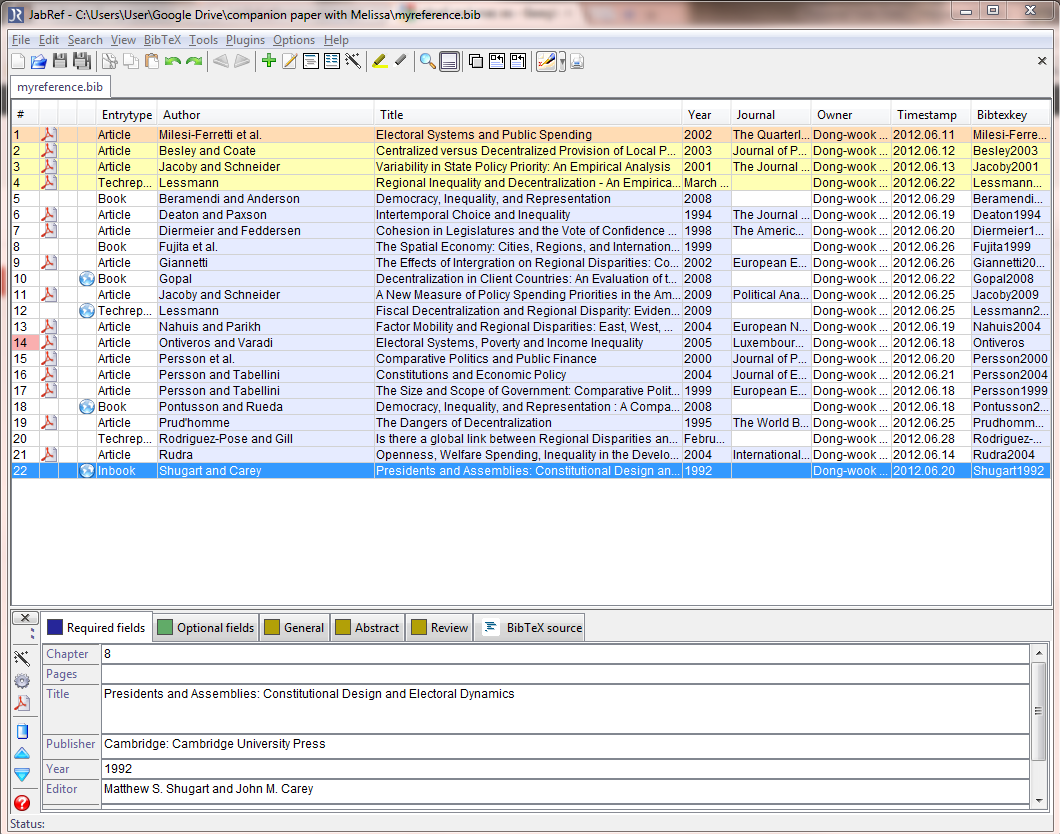
\includegraphics[width=9cm]{img/jabref} % image de X cm de large
%\caption{Titre de la figure} %titre de la figure
%\label{titre_fig} %label de la figure (ex voir figure W)
\end{figure} %fin de l'environnement figure

\vspace*{-0.5cm}
{\footnotesize Téléchargement: http://jabref.sourceforge.net/ }

\end{frame}


%%%%%%%%%%%%%%%%%%%%%%%%%%%%%%
%%%%%%%%%%% PART%% %%%%%%%%%%%%%%
%%%%%%%%%%%%%%%%%%%%%%%%%%%%%%


\part{Commandes avancées}

\section{Commandes personnalisées}

\begin{frame}[fragile]
	\frametitle{Créer ses propres commandes}
	Pourquoi?
	\begin{itemize}
		\item Réutilisation
		\item Simplification
	\end{itemize}
	
	Définition

	\begin{lstlisting}
\newcommand{\ltsname}{Labeled Transition System}
\newcommand{\abs}[1]{\left|#1\right|}
\newcommand{\lts}[1][]{\left(Q^{#1},q_0^{#1},A_{#1},\rightarrow_{#1}\right)}
	\end{lstlisting}
	Utilisation
		\begin{itemize}
	\item \lstinline?\ltsname? $\Rightarrow$ \ltsname
	\item \lstinline?\abs{\pi}? $\Rightarrow$ $\abs{\pi}$
	\item \lstinline?\lts? $\Rightarrow$ $\lts$\\
		\lstinline?\lts[n]? $\Rightarrow$ $\lts[n]$
	\end{itemize}
	Restrictions
	\begin{itemize}
		\item Pas de chiffres
		\item Pas de @
	\end{itemize}
\end{frame}

\begin{frame}[fragile]
	\frametitle{Redéfinir des commandes}

	\begin{lstlisting}
\renewcommand{\vec}[1]{\overrightarrow{#1}}
	\end{lstlisting}
	Utilisation
		\begin{itemize}
	\item \lstinline?\vec{AB}? $\Rightarrow$ $\vec{AB}$
	\end{itemize}

\end{frame}

\section{Comprendre la compilation}

\begin{frame}
	\frametitle{Fichiers auxiliaires}
	\begin{description}
	\item[log] fichier où \LaTeX{} écrit tout un tas d'informations sur la dernière compilation
	\item[aux] fichier auxiliaire: stocke les références, citations, numéros de page, etc.
	\item[toc] fichier contenant la table des matières
	\item[lof] fichier contenant la liste des figures
	\item[lot] fichier contenant la liste des tables
	\item[bbl] fichier contenant la bibliographie
	\end{description}
\end{frame}

\setbeamercovered{transparent}
\begin{frame}
\frametitle{Cycle de compilation}
\begin{center}
    \begin{tikzpicture}[every node/.style={shape=rectangle, shape aspect=1.61, rounded corners},
                        every path/.style={thick, >=triangle 60},
                        file/.style={minimum height=0.8cm, minimum width=1.29, fill=blue!20, draw=blue},
                        bin/.style={minimum width=2.42cm, minimum height=1.5cm, fill=red!20, draw=red}]
                        \only<1, 3-4>{\node[bin] (bin) at (0,0) {\LaTeX{}};}
                        \only<2>{\node[bin] (bin) at (0,0) {Bib\TeX{}};}
                        \onslide<1, 3-4>{\node[file] (tex) at (-3, 1) {\texttt{.tex}};}
                        \onslide<2>{\node[file] (bib) at (-3, 0) {\texttt{.bib}};}
                        \onslide<3-4>{\node[file] (bst) at (-3, -1) {\texttt{.bst}};}

                        \onslide<3-4>{\node[file] (pdf) at (3,0.75) {\texttt{.pdf}};}
                        \onslide<1, 3-4>{\node[file] (log) at (3, -0.75) {\texttt{.log}};}

                        \onslide<2-4>{\node[file] (aux) at (-1.5, 2) {\texttt{.aux}};}
                        \onslide<3-4>{\node[file] (bbl) at (0, 2) {\texttt{.bbl}};}
                        \onslide<2>{\node[file] (blg) at (1.5, 2) {\texttt{.blg}};}

                        \onslide<4>{\node[file] (toc) at (-1.5, -2) {\texttt{.toc}};}
                        \onslide<4>{\node[file] (lof) at (0, -2) {\texttt{.lof}};}
                        \onslide<4>{\node[file] (lot) at (1.5, -2) {\texttt{.lot}};}

                        \only<1>{
                            \draw[->] (tex) -- (bin);
                            \draw[->] (bin) -- (log);
                            \draw[->] (bin) -- (pdf);
                            \draw[->] (bin) -- (aux);
                        }
                        \only<2>{
                            \draw[->] (bib) -- (bin);
                            \draw[->] (aux) -- (bin);
                            \draw[->] (bin) -- (blg);
                            \draw[->] (bin) -- (bbl);
                        }
                        \only<3>{
                            \draw[->] (tex) -- (bin);
                            \draw[->] (aux) -- (bin);
                            \draw[->] (bst) -- (bin);
                            \draw[->] (bbl) -- (bin);
                            \draw[->] (bin) -- (log);
                            \draw[->] (bin) -- (pdf);
                            \draw[->] (bin) -- (toc);
                            \draw[->] (bin) -- (lof);
                            \draw[->] (bin) -- (lot);
                        }
                        \only<4>{
                            \draw[->] (tex) -- (bin);
                            \draw[->] (aux) -- (bin);
                            \draw[->] (bst) -- (bin);
                            \draw[->] (bbl) -- (bin);
                            \draw[->] (bin) -- (log);
                            \draw[->] (bin) -- (pdf);
                            \draw[<-] (bin) -- (toc);
                            \draw[<-] (bin) -- (lof);
                            \draw[<-] (bin) -- (lot);
                        }
    \end{tikzpicture}
\end{center}
\end{frame}

\setbeamercovered{invisible}
%%%%%%%%%%%%%%%%%%%%%%%%%%%%%%
%%%%%%%%%%% SECTION %%%%%%%%%%%%%%
%%%%%%%%%%%%%%%%%%%%%%%%%%%%%%

\section{Autres éditeurs \LaTeX}


%%%%%%%%% SLIDE %%%%%%%%%%%%%%%%%%

\begin{frame}{Texniccenter}

\begin{figure} %debut de l'environnement figure
\centering %figure centree
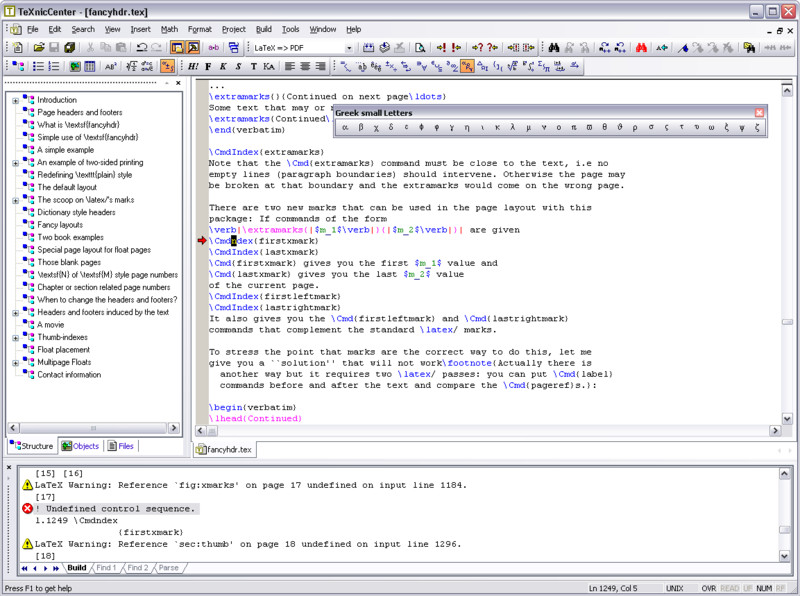
\includegraphics[width=9cm]{img/Texniccenter} % image de X cm de large
%\caption{Titre de la figure} %titre de la figure
%\label{titre_fig} %label de la figure (ex voir figure W)
\end{figure} %fin de l'environnement figure

{\footnotesize Téléchargement: http://www.texniccenter.org/ }

\end{frame}


%%%%%%%%% SLIDE %%%%%%%%%%%%%%%%%%

\begin{frame}{LyX}

\begin{figure} %debut de l'environnement figure
\centering %figure centree
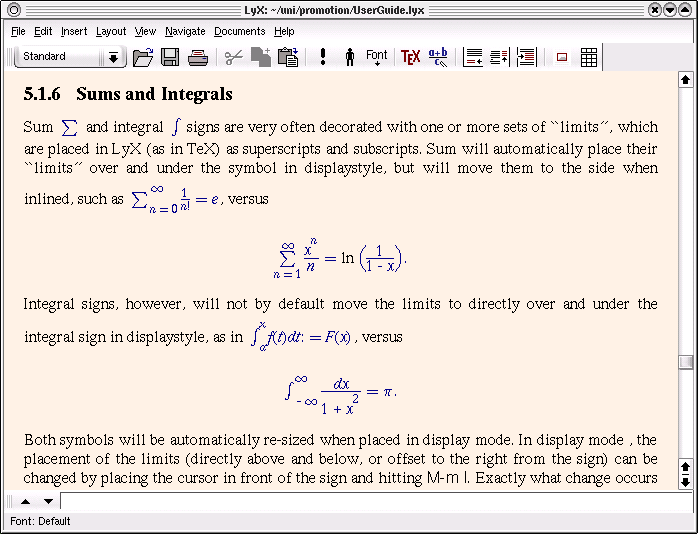
\includegraphics[width=8cm]{img/LyXScreen_Linux_en} % image de X cm de large
%\caption{Titre de la figure} %titre de la figure
%\label{titre_fig} %label de la figure (ex voir figure W)
\end{figure} %fin de l'environnement figure

{\footnotesize Téléchargement: http:// 	www.lyx.org/ }

\end{frame}


%%%%%%%%% SLIDE %%%%%%%%%%%%%%%%%%

\begin{frame}{Texmaker}

\begin{figure} %debut de l'environnement figure
\centering %figure centree
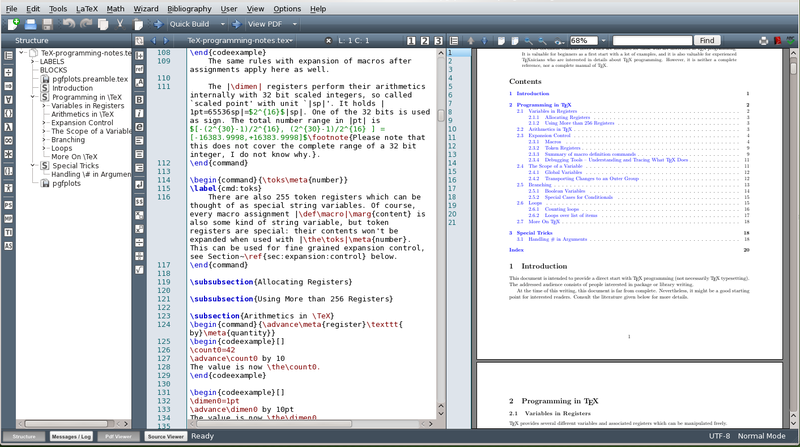
\includegraphics[width=9cm]{img/TexmakerView} % image de X cm de large
%\caption{Titre de la figure} %titre de la figure
%\label{titre_fig} %label de la figure (ex voir figure W)
\end{figure} %fin de l'environnement figure

{\footnotesize Téléchargement: http://www.xm1math.net/texmaker/ }

\end{frame}


%%%%%%%%%%%%%%%%%%%%%%%%%%%%%%
%%%%%%%%%%% PART%% %%%%%%%%%%%%%%
%%%%%%%%%%%%%%%%%%%%%%%%%%%%%%

\part{Inclusion de figures à l'aide de différents outils}

%TikZ
% Présentation de TikZ

\section{Présentation de PGF/TikZ}

\begin{frame}
  \frametitle{PGF/TikZ : du dessin vectoriel en \LaTeX}

Qu'est-ce que PGF/TikZ ?
\begin{itemize}
  \item PGF est un langage complet et compliqué de dessin vectoriel,
  \item TikZ est une surcouche plus simple pour utiliser PGF.
\end{itemize}

\bigskip
Ils permettent de dessiner des figures facilement. Beaucoup d'avantages :
\begin{itemize}
  \item les figures sont intégrés au document \LaTeX{} (pas de fichier externe),
  \item dessin vectoriel : toujours lisse, quel que soit le niveau de zoom,
  \item très riche, beaucoup d'exemples disponibles faciles à reprendre.
\end{itemize}

\bigskip
Inconvénients :
\begin{itemize}
  \item parfois difficile à prendre en main,
  \item peut alourdir la compilation et le fichier final,
  \item ne permet pas de tout faire (mais presque).
\end{itemize}
\end{frame}



\section{Quelques exemples avec TikZ}

\def \tikzexa
{
\begin{tikzpicture}[
	scale=0.75,
	start chain=1 going below, 
	start chain=2 going right,
	node distance=1mm,
	desc/.style={
		scale=0.75,
		on chain=2,
		rectangle,
		rounded corners,
		draw=black, 
		very thick,
		text centered,
		text width=8cm,
		minimum height=12mm,
		fill=blue!30
		},
	it/.style={
		fill=blue!10
	},
	level/.style={
		scale=0.75,
		on chain=1,
		minimum height=12mm,
		text width=2cm,
		text centered
	},
	every node/.style={font=\sffamily}
]

% Levels
\node [level] (Level 5) {Level 5};
\node [level] (Level 4) {Level 4};
\node [level] (Level 3) {Level 3};
\node [level] (Level 2) {Level 2};
\node [level] (Level 1.5) { };
\node [level] (Level 1) {Level 1};
\node [level] (Level 0) {Level 0};

% Descriptions
\chainin (Level 5); % Start right of Level 5
% IT levels
\node [desc, it] (Archives) {Archives/File Servers};
\node [desc, it, continue chain=going below] (ERP) {ERP/Finance/Messaging};
% ICS levels
\node [desc] (Operations) {Operations Management/Historians};
\node [desc] (Supervisory) {Supervisory Controls};
\node [desc, text width=3.5cm, xshift=2.25cm] (PLC) {PLC/RTU IP Communication};
\node [desc, text width=3.5cm, xshift=-4.5cm] (SIS) {Safety Instrumented Systems};
\node [desc, xshift=2.25cm] (IO) {I/O from Sensors};
\end{tikzpicture}
}






\def \tikzexb
{
\begin{tikzpicture}
\draw[gray,fill=gray,path fading=south] (0,0) rectangle +(0.3,-0.3);% <- MAGIC
  % (if this is not present none of the shadings work)

%top
\shade[left color=black!10!white,right color=black!40!white] (-1,0.75)
  -- ++(2,0) -- ++(0.25,-0.25) -- ++(-2.5,0) -- cycle;
\draw (-1,0.75) -- ++(2,0) -- ++(0.25,-0.25) -- ++(-2.5,0) -- cycle;

%source
\shade[left color=black!10!white,right color=black!40!white] (1.25,0.5)
  -- ++(0,-1.75) -- ++(-2.5,0) -- ++(0,1.75) -- cycle;
\draw (1.25,0.5) -- ++(0,-1.75) -- ++(-2.5,0) -- ++(0,1.75) -- cycle;

%top condenser system
\shade[left color=black!10!white,right color=black!40!white] (1.25,-1.25)
  -- ++(0.25,-0.25) -- ++(-3,0) -- ++(0.25,0.25) -- cycle;
\draw (1.25,-1.25) -- ++(0.25,-0.25) -- ++(-3,0) -- ++(0.25,0.25) -- cycle;

%condenser system
\shade[left color=black!10!white,right color=black!40!white] (1.5,-1.5)
  -- ++(0,-2) -- ++(-3,0) -- ++(0,2) -- cycle;
\draw (1.5,-1.5) -- ++(0,-2) -- ++(-3,0) -- ++(0,2) -- cycle;

%condenser bottom
\shade[left color=black!10!white,right color=black!40!white] (1.5,-3.5)
  -- ++(-0.25,-0.25) -- ++(-2.5,0) -- ++(-0.25,0.25) -- cycle;
\draw (1.5,-3.5) -- ++(-0.25,-0.25) -- ++(-2.5,0) -- ++(-0.25,0.25) -- cycle;

%specimen and objective
\shade[left color=black!10!white,right color=black!40!white] (1.25,-3.75)
  -- ++(0,-2.5) -- ++(-2.5,0) -- ++(0,2.5) -- cycle;
\draw (1.25,-3.75) -- ++(0,-2.5) -- ++(-2.5,0) -- ++(0,2.5) -- cycle;

%projector system top
\shade[left color=black!10!white,right color=black!40!white] (1.25,-6.25)
  -- ++(0.25,-0.25) -- ++(-3,0) -- ++(0.25,0.25) -- cycle;
\draw (1.25,-6.25) -- ++(0.25,-0.25) -- ++(-3,0) -- ++(0.25,0.25) -- cycle;

%projector system
\shade[left color=black!10!white,right color=black!40!white] (1.5,-6.5)
  -- ++(0,-1.5) -- ++(-3,0) -- ++(0,1.5) -- cycle;
\draw (1.5,-6.5) -- ++(0,-1.5) -- ++(-3,0) -- ++(0,1.5) -- cycle;

%image
\shade[left color=black!10!white,right color=black!40!white] (1.5,-8)
  -- ++(1,-1.5) -- ++(0,-0.75) -- ++(-5,0) -- ++(0,0.75) -- ++(1,1.5) -- cycle;
\draw (1.5,-8) -- ++(1,-1.5) -- ++(0,-0.75) -- ++(-5,0) -- ++(0,0.75)
  -- ++(1,1.5) -- cycle;

%sample entrance
\shade[left color=black!10!white,right color=black!40!white] (-1.25,-4.5)
  -- ++(-0.5,0) -- ++(-0.2,-0.2) -- ++(0,-0.6) -- ++(0.2,-0.2)
  -- ++(0.5,0) -- cycle;
\draw (-1.25,-4.5) -- ++(-0.5,0) -- ++(-0.2,-0.2) -- ++(0,-0.6)
  -- ++(0.2,-0.2)  -- ++(0.5,0) -- cycle;

%sample holder
\draw[fill=black] (-1.95,-4.8) -- ++(-0.08,0) -- ++(-0.02,-0.02)
  -- ++(0,-0.36) -- ++(0.02,-0.02) -- ++(0.08,0) -- cycle;

%inside
\begin{scope}
  \path[clip,decoration={random steps, segment length=6pt, amplitude=2pt},
	  decorate] (0,0.5) -- ++(0.4,0) -- ++(0.4,-0.4) -- ++(0,-8.5)
	  -- ++(1,-1.3) -- ++(-0.4,-0.4) -- ++(-2.8,0) -- ++(-0.4,0.4)
	  -- ++(1,1.3) -- ++(0,8.5) -- ++(0.4,0.4) -- cycle;
  \shade[left color=black!40!white,right color=black!10!white] (-1,0.75)
	  -- ++(2,0) -- ++(0.25,-0.25) -- ++(0,-1.75) -- ++(0.25,-0.25) -- ++(0,-2)
	  -- ++(-0.25,-0.25) -- ++(0,-2.5) -- ++(0.25,-0.25) -- ++(0,-1.5)
	  -- ++(1,-1.5) -- ++(0,-0.75) -- ++(-5,0) -- ++(0,0.75) -- ++(1,1.5)
	  -- ++ (0,1.5) -- ++(0.25,0.25) -- ++(0,2.5) -- ++(-0.25,0.25) -- ++(0,2)
	  -- ++(0.25,0.25) -- ++(0,1.75) -- cycle;

%source
\draw (-0.25,0.15) -- ++(0,-0.05) .. controls +(0,-0.08) and +(-0.08,0)
  .. ++(0.1,-0.1) -- ++(0.05,0) .. controls +(0.08,0) and +(0,0.08)
  .. ++(0.1,-0.1) .. controls +(0,0.08) and +(-0.08,0) .. ++(0.1,0.1) --
  ++(0.05,0) .. controls +(0.08,0) and +(0,-0.08) .. ++(0.1,0.1) -- ++(0,0.05);

%C1
\draw[fill=brown!80!yellow] (-0.4,-1.75) -- ++(-0.5,0) -- ++(0,-0.5)
  -- ++(0.5,0) -- cycle;
\draw (-0.4,-1.75) ++(-0.04,-0.04) -- ++(-0.42,0) -- ++(0,-0.42)
  -- ++(0.42,0) -- cycle;
\begin{scope}
  \path[clip,draw] (-0.4,-1.75) ++(-0.04,-0.04) -- ++(-0.42,0)
	  -- ++(0,-0.42) -- ++(0.42,0) -- cycle;
  \foreach \j in {-0.07,-0.14,...,-0.42}
	  \foreach \i in {-0.07,-0.14,...,-0.42} {
		  \draw[fill=brown!40!yellow] (-0.4,-1.75) ++(-0.04,-0.04)
			  ++(0.035,0.035) ++(\i,\j) circle (0.035);
	  }
\end{scope}
\draw[fill=brown!80!yellow] (0.9,-1.75) -- ++(-0.5,0) -- ++(0,-0.5)
  -- ++(0.5,0) -- cycle;
\draw (0.9,-1.75) ++(-0.04,-0.04) -- ++(-0.42,0) -- ++(0,-0.42)
  -- ++(0.42,0) -- cycle;
\begin{scope}
  \path[clip,draw] (0.9,-1.75) ++(-0.04,-0.04) -- ++(-0.42,0)
	  -- ++(0,-0.42) -- ++(0.42,0) -- cycle;
  \foreach \j in {-0.07,-0.14,...,-0.42}
	  \foreach \i in {-0.07,-0.14,...,-0.42} {
		  \draw[fill=brown!40!yellow] (0.9,-1.75) ++(-0.04,-0.04)
			  ++(0.035,0.035) ++(\i,\j) circle (0.035);
	  }
\end{scope}

%C2
\draw[fill=brown!80!yellow] (-0.4,-2.75) -- ++(-0.5,0) -- ++(0,-0.5)
  -- ++(0.5,0) -- cycle;
\draw (-0.4,-2.75) ++(-0.04,-0.04) -- ++(-0.42,0) -- ++(0,-0.42)
  -- ++(0.42,0) -- cycle;
\begin{scope}
  \path[clip,draw] (-0.4,-2.75) ++(-0.04,-0.04) -- ++(-0.42,0)
	  -- ++(0,-0.42) -- ++(0.42,0) -- cycle;
  \foreach \j in {-0.07,-0.14,...,-0.42}
	  \foreach \i in {-0.07,-0.14,...,-0.42} {
		  \draw[fill=brown!40!yellow] (-0.4,-2.75) ++(-0.04,-0.04)
			  ++(0.035,0.035) ++(\i,\j) circle (0.035);
	  }
\end{scope}
\draw[fill=brown!80!yellow] (0.9,-2.75) -- ++(-0.5,0) -- ++(0,-0.5)
  -- ++(0.5,0) -- cycle;
\draw (0.9,-2.75) ++(-0.04,-0.04) -- ++(-0.42,0) -- ++(0,-0.42)
  -- ++(0.42,0) -- cycle;
\begin{scope}
  \path[clip,draw] (0.9,-2.75) ++(-0.04,-0.04) -- ++(-0.42,0)
	  -- ++(0,-0.42) -- ++(0.42,0) -- cycle;
  \foreach \j in {-0.07,-0.14,...,-0.42}
	  \foreach \i in {-0.07,-0.14,...,-0.42} {
		  \draw[fill=brown!40!yellow] (0.9,-2.75) ++(-0.04,-0.04)
			  ++(0.035,0.035) ++(\i,\j) circle (0.035);
	  }
\end{scope}

%condenser aperture
\draw[fill=black] (-1,-3.45) -- ++(0.6,0) -- ++(-0.1,-0.1)
  -- ++(-0.5,0) -- cycle;
\draw[fill=black] (1,-3.45) -- ++(-0.6,0) -- ++(0.1,-0.1)
  -- ++(0.5,0) -- cycle;

%specimen
\draw[fill=brown!70!yellow] (-1,-4.95) -- ++(0.75,0) -- ++(0.05,-0.045)
  -- ++(0,-0.01) -- ++(-0.05,-0.045) -- ++(-0.75,0) -- cycle;
\draw[fill=black] (-0.2,-4.995) -- ++(0.4,0) -- ++(0,-0.01)
  -- ++(-0.4,0) -- cycle;
  
%objective
\draw[fill=brown!80!yellow] (-0.4,-5.25) -- ++(-0.5,0) -- ++(0,-0.5)
  -- ++(0.5,0) -- cycle;
\draw (-0.4,-5.25) ++(-0.04,-0.04) -- ++(-0.42,0) -- ++(0,-0.42)
  -- ++(0.42,0) -- cycle;
\begin{scope}
  \path[clip,draw] (-0.4,-5.25) ++(-0.04,-0.04) -- ++(-0.42,0)
	  -- ++(0,-0.42) -- ++(0.42,0) -- cycle;
  \foreach \j in {-0.07,-0.14,...,-0.42}
	  \foreach \i in {-0.07,-0.14,...,-0.42} {
		  \draw[fill=brown!40!yellow] (-0.4,-5.25) ++(-0.04,-0.04)
			  ++(0.035,0.035) ++(\i,\j) circle (0.035);
	  }
\end{scope}
\draw[fill=brown!80!yellow] (0.9,-5.25) -- ++(-0.5,0) -- ++(0,-0.5)
  -- ++(0.5,0) -- cycle;
\draw (0.9,-5.25) ++(-0.04,-0.04) -- ++(-0.42,0) -- ++(0,-0.42)
  -- ++(0.42,0) -- cycle;
\begin{scope}
  \path[clip,draw] (0.9,-5.25) ++(-0.04,-0.04) -- ++(-0.42,0)
	  -- ++(0,-0.42) -- ++(0.42,0) -- cycle;
  \foreach \j in {-0.07,-0.14,...,-0.42}
	  \foreach \i in {-0.07,-0.14,...,-0.42} {
		  \draw[fill=brown!40!yellow] (0.9,-5.25) ++(-0.04,-0.04)
			  ++(0.035,0.035) ++(\i,\j) circle (0.035);
	  }
\end{scope}
  
%objective aperture
\draw[fill=black] (-1,-5.95) -- ++(0.7,0) -- ++(-0.1,-0.1)
  -- ++(-0.6,0) -- cycle;
\draw[fill=black] (1,-5.95) -- ++(-0.7,0) -- ++(0.1,-0.1)
  -- ++(0.6,0) -- cycle;
  
  

%projector system
\draw[fill=brown!80!yellow] (-0.4,-6.75) -- ++(-0.5,0)
  -- ++(0,-1) -- ++(0.5,0) -- cycle;
\draw (-0.4,-6.75) ++(-0.04,-0.04) -- ++(-0.42,0) -- ++(0,-0.92)
  -- ++(0.42,0) -- cycle;
\begin{scope}
  \path[clip,draw] (-0.4,-6.75) ++(-0.04,-0.04) -- ++(-0.42,0)
	  -- ++(0,-0.92) -- ++(0.42,0) -- cycle;
  \foreach \j in {-0.07,-0.14,...,-0.92}
	  \foreach \i in {-0.07,-0.14,...,-0.42} {
		  \draw[fill=brown!40!yellow] (-0.4,-6.75) ++(-0.04,-0.04)
			  ++(0.035,0.035) ++(\i,\j) circle (0.035);
	  }
\end{scope}
\draw[fill=brown!80!yellow] (0.9,-6.75) -- ++(-0.5,0) -- ++(0,-1)
  -- ++(0.5,0) -- cycle;
\draw (0.9,-6.75) ++(-0.04,-0.04) -- ++(-0.42,0) -- ++(0,-0.92)
  -- ++(0.42,0) -- cycle;
\begin{scope}
  \path[clip,draw] (0.9,-6.75) ++(-0.04,-0.04) -- ++(-0.42,0)
	  -- ++(0,-0.92) -- ++(0.42,0) -- cycle;
  \foreach \j in {-0.07,-0.14,...,-0.92}
	  \foreach \i in {-0.07,-0.14,...,-0.42} {
		  \draw[fill=brown!40!yellow] (0.9,-6.75) ++(-0.04,-0.04)
			  ++(0.035,0.035) ++(\i,\j) circle (0.035);
	  }
\end{scope}

%image
\draw[fill=gray] (2,-10) -- ++(0,-0.2) -- ++(-4,0) -- ++(0,0.2) -- cycle;
  
%beam
\draw[blue] (0,-0.1) ++(260:0.3) -- (-0.3,-2) -- ++(0.6,-1) -- ++(-0.3,-2)
  -- ++(-0.3,-0.5) -- ++(0.35,-1.25);
\draw[blue] (0,-0.1) ++(280:0.3) -- (0.3,-2) -- ++(-0.6,-1) -- ++(0.3,-2)
  -- ++(0.3,-0.5) -- ++(-0.35,-1.25);
\draw[blue] (-0.3,-7.75) -- ++(-1,-2.25);
\draw[blue] (0.3,-7.75) -- ++(1,-2.25);
\draw[blue,dash pattern=on 4pt off 1pt on 1pt off 1pt on 1pt off 1pt]
  (0,-0.4) -- (0,-10);

\end{scope}

%labels
\draw (2,0) node[right] {source};
\draw (-2,-2) node[left] {C1};
\draw (-2,-3) node[left] {C2};
\draw (-2,-3.5) node[left] {condenser aperture};
\draw (2,-2.5) node[right] {condenser system};
\draw (2,-5) node[right] {sample};
\draw (-2.3,-5) node[left] {sample holder};
\draw (2,-5.5) node[right] {objective lens};
\draw (2,-6) node[right] {objective aperture};
\draw (2,-7.25) node[right] {projector system};
\draw (3,-10) node[right] {imaging};
\end{tikzpicture}
}






\def \tikzexc
{
\begin{tikzpicture}[->,>=stealth',shorten >=1pt,auto,node distance=3cm,
  thick,main node/.style={circle,fill=blue!20,draw,font=\sffamily\Large\bfseries}]

  \node[main node] (1) {1};
  \node[main node] (2) [below left of=1] {2};
  \node[main node] (3) [below right of=2] {3};
  \node[main node] (4) [below right of=1] {4};

  \path[every node/.style={font=\sffamily\small}]
    (1) edge node [left] {0.6} (4)
        edge [bend right] node[left] {0.3} (2)
        edge [loop above] node {0.1} (1)
    (2) edge node [right] {0.4} (1)
        edge node {0.3} (4)
        edge [loop left] node {0.4} (2)
        edge [bend right] node[left] {0.1} (3)
    (3) edge node [right] {0.8} (2)
        edge [bend right] node[right] {0.2} (4)
    (4) edge node [left] {0.2} (3)
        edge [loop right] node {0.6} (4)
        edge [bend right] node[right] {0.2} (1);
\end{tikzpicture}
}







\def \tikzexd
{
\begin{tikzpicture}[
    media/.style={font={\footnotesize\sffamily}},
    wave/.style={
        decorate,decoration={snake,post length=1.4mm,amplitude=2mm,
        segment length=2mm},thick},
    interface/.style={
        % The border decoration is a path replacing decorator. 
        % For the interface style we want to draw the original path.
        % The postaction option is therefore used to ensure that the
        % border decoration is drawn *after* the original path.
        postaction={draw,decorate,decoration={border,angle=-45,
                    amplitude=0.3cm,segment length=2mm}}},
    ]
    % Round rectangle
    \fill[gray!10,rounded corners] (-4,-3) rectangle (4,0);
    % Interface
    \draw[blue,line width=.5pt,interface](-4,0)--(4,0);
    % Vertical dashed line
    \draw[dashed,gray](0,-3)--(0,3);
    % Coordinates system
    \draw(0,0.15)node[above]{$x$};
    \draw[<->,line width=1pt] (1,0) node[above]{$y$}-|(0,-1) node[left]{$z$};
    % Incidence
    \draw[->,wave]
         (135:3.2cm)--(135:2.5cm)node[right]{$f^0$};
    \draw[gray](0:0cm)--(135:2cm);
    \path (0,0)++(113:1cm)node{$\phi$};
    \draw[->](0,0.75)arc(90:135:.75cm);
    % Transmission
    \draw[->,wave]
         (-30:2.5cm)--(-30:3.2cm)node[right]{$f^+$};
    \draw[gray](0:0cm)--(-30:2cm);
    \path (0,0)++(-60:1cm)node{$\theta$};
    \draw[->] (0,-0.75) arc (-90:-30:.75cm);
    % Reflection
    \draw[->,wave]
         (45:2.5cm)--(45:3.2cm)node[right]{$f^-$};
    \path (0,0)++(-22:1.75cm) node{$\psi$};
    \draw[gray](0:0cm)--(45:2cm);
    \draw[->] (0,-1.5)arc(-90:45:1.5cm);
    % Media names
    \path[media] (-3,.6)  node {media 1}
                 (-3,-.6) node {media 2};

    % $x$ axis
    \filldraw[fill=white,line width=1pt](0,0)circle(.12cm);
    \draw[line width=.6pt] (0,0)
                          +(-135:.12cm) -- +(45:.12cm)
                          +(-45:.12cm) -- +(135:.12cm);
    % Interface pointer
    \draw[-latex,thick](3.2,0.5)node[right]{$\mathsf{S_{1,2}}$}
         to[out=180,in=90] (3,0);
    % To-paths are really useful for drawing curved lines. The above
    % to path is equal to:
    %
    % \draw[-latex,thick](3.2,0.5)node[right]{$\mathsf{S_{1,2}}$}
    %      ..controls +(180:.2cm) and +(up:0.25cm) .. (3,0);
    % Internally the to path is translated to a similar bezier curve,
    % but the to path syntax hides the complexity from the user. 
\end{tikzpicture}
}

\begin{frame}
  \begin{figure}
    \centering
    \tikzexa
    \caption{\footnotesize Modèle d'architecture --- TEXample.net \cite{tikzandpgfexamples}}
  \end{figure}
\end{frame}

\begin{frame}
  \begin{figure}
    \centering
    \tikzexc
    \caption{\footnotesize Graphe simple --- TEXample.net \cite{tikzandpgfexamples}}
  \end{figure}
\end{frame}

\begin{frame}
  \begin{figure}
    \centering
    \scalebox{0.7}{\tikzexe}
    \caption{\footnotesize Circuit électrique --- TEXample.net \cite{tikzandpgfexamples}}
  \end{figure}
\end{frame}

\begin{frame}
  \begin{figure}
    \centering
    \scalebox{0.7}{\tikzexd}
    \caption{\footnotesize Incidence oblique --- TEXample.net \cite{tikzandpgfexamples}}
  \end{figure}
\end{frame}

\begin{frame}
  \begin{figure}
    \centering
    \scalebox{0.7}{\tikzexb}
    \caption{\footnotesize Microscope électronique à transmission --- TEXample.net \cite{tikzandpgfexamples}}
  \end{figure}
\end{frame}



\section{Utilisation de TikZ}

\begin{frame}[fragile]
  \frametitle{Préambule et création d'une figure}

TikZ doit être chargé dans le préambule :
\lstinline?\usepackage{tikz}?

\medskip
On peut aussi charger des bibliothèques propres à TikZ dans le préambule avec :
\lstinline?\usetikzlibrary{bibliotheques}?,
ce qui permet d'utiliser :
\begin{itemize}
  \item de nouvelles formes de pointes de flèches (\lstinline?arrows?),
  \item des dégradés (\lstinline?shadings?),
  \item des styles de lignes (\lstinline?decorations.pathmorphing?), ...
\end{itemize}

\bigskip
Dans le document, on définit une image TikZ à l'aide de l'environnement \lstinline?tikzpicture?,
souvent inclus dans une \lstinline?figure? :

\begin{lstlisting}
\begin{figure}
  \begin{tikzpicture}
    ...
    ...    % Contenu de l'image
    ...
  \end{tikzpicture}
  \caption{...}
\end{figure}
\end{lstlisting}
\end{frame}




\def \tikzexnodes
{
\node[circle, fill=yellow, draw]
  (rond) {1};
\node[ellipse, fill=red!50]
  (ellipse) [right of=1, node distance=3cm] {Une ellipse};
\node[diamond, fill=blue!50, draw=blue, thick]
  (diamantvide) [left of=1, node distance=2cm] {};
}

\def \tikzexedges
{
\path[->] (rond) edge (ellipse);
\path[o->, bend right] (rond) edge (diamantvide);
\path[o->>, bend right] (diamantvide) edge
  node[below, fill=green!30] (retour) {retour}
  (rond);
\path[-, bend right] (retour.east) edge (rond.south);
}

\begin{frame}[fragile,t]
  \frametitle{Exemple : un graphe simple}

\begin{figure}
  \begin{tikzpicture}
    \tikzexnodes
    \tikzexedges
  \end{tikzpicture}
\end{figure}

Une figure TikZ est constituée d'éléments définis à l'aide de commandes :

\begin{lstlisting}
  \commande[param£\`e£tres] ... suite de la commande ... ;
\end{lstlisting}

Par exemple, un graphe est composé de nœuds et d'arcs entre ces nœuds.
Tous sont définis à l'aide de commandes TikZ.

\medskip
On commence par définir une figure et une image TikZ :
\begin{lstlisting}
\begin{figure}
  \begin{tikzpicture}
    ...    % La figure ici
  \end{tikzpicture}
\end{figure}
\end{lstlisting}
\end{frame}

\begin{frame}[fragile, t]
  \frametitle{Exemple : un graphe simple}

\begin{figure}
  \begin{tikzpicture}
    \tikzexnodes
  \end{tikzpicture}
\end{figure}

On définit un nœud avec la commande \lstinline?\node? et on peut spécifier :
\medskip
\begin{itemize}
  \item le nom interne \lstinline?(nom)? et l'étiquette visible \lstinline?{etiquette}?
  \item la forme \quad \lstinline?circle?, \lstinline?ellipse?, \lstinline?square?, \lstinline?diamond?
  \item le type de ligne \quad \lstinline?draw? : visible, \lstinline?draw=blue? : en bleu, \lstinline?thick? : en gras
  \item la couleur de fond \quad \lstinline?fill=yellow? : fond jaune, \lstinline?shading? : dégradé
  \item la position \quad \lstinline?left/right/above/below of=n? : position par rapport à \lstinline?n?
\end{itemize}

\begin{lstlisting}
\node[circle, fill=yellow, draw]
  (rond) {1};
\node[ellipse, fill=red!50]
  (ellipse) [right of=1, node distance=3cm] {Une ellipse};
\node[diamond, fill=blue!50, draw=blue, thick]
  (diamantvide) [left of=1, node distance=2cm] {};
\end{lstlisting}
\end{frame}

\begin{frame}[fragile, t]
  \frametitle{Exemple : un graphe simple}

\begin{figure}
  \begin{tikzpicture}
    \tikzexnodes
    \tikzexedges
  \end{tikzpicture}
\end{figure}

On définit ensuite un arc entre deux nœuds avec la commande

\begin{lstlisting}
    \path[£\meta{options}£] (£\meta{origine}£) edge (£\meta{cible}£);
\end{lstlisting}

On peut définir le type de flèche (\lstinline?->?, \lstinline?o->?, \lstinline?-?),
la courbure (\lstinline?bend right?),
etc.

\begin{lstlisting}
\path[->] (rond) edge (ellipse);
\path[o->, bend right] (rond) edge (diamantvide);
\end{lstlisting}

On peut placer un nouveau nœud sur un arc avec le mot-clef \lstinline?node?.

\begin{lstlisting}
\path[-, bend right] (retour.east) edge (rond.south);
\path[o->>, bend right] (diamantvide) edge
  node[below, fill=green!30] (retour) {retour} (rond);
\end{lstlisting}
\end{frame}



\section{Conclusion sur TikZ}

\begin{frame}
  \frametitle{Réutiliser au maximum}

Pour produire de belles figures TikZ, le mieux est de chercher des exemples et de les modifier.

\begin{center}
Pour cela : \Huge Internet !
\end{center}

On pourra notamment se servir des exemples de TEXample.net \cite{tikzandpgfexamples}.

\bigskip
De plus, il est possible de :
\begin{itemize}
  \item définir des thèmes pour des figures semblables,
  \item d'utiliser des bibliothèques pour des diagrammes répandus (UML, schémas électriques...).
\end{itemize}
\end{frame}


% Beamer


%%%%%%%%%%%%%%%%%%%%%%%%%%%%%%
%%%%%%%%%%% PART%% %%%%%%%%%%%%%%
%%%%%%%%%%%%%%%%%%%%%%%%%%%%%%

\part{Beamer}

%%%%%%%%%%%%%%%%%%%%%%%%%%%%%%
%%%%%%%%%%% SECTION %%%%%%%%%%%%%%
%%%%%%%%%%%%%%%%%%%%%%%%%%%%%%

\section{Utilisation de Beamer}

%%%%%%%%% SLIDE %%%%%%%%%%%%%%%%%%

\begin{frame}[fragile]
  \frametitle{Qu'est-ce que Beamer ?}

Beamer est une classe \LaTeX{} :

\lstinline?\documentclass{beamer}?

\medskip
Points communs :
\begin{itemize}
  \item structuration (parties, sections, sous-sections ; pas de chapitres),
  \item mise en forme du texte,
  \item inclusion de figures et de formules mathématiques,
  \item etc.
\end{itemize}

\medskip
Différences :
\begin{itemize}
  \item structuration en diapositives,
  \item nouvelles commandes (transitions),
  \item mise en page différente (police, agencement).
\end{itemize}
\end{frame}



\begin{frame}[fragile]
  \frametitle{Définition du document}

Beamer est une classe \LaTeX{} :

\lstinline?\documentclass[options]{beamer}?

\medskip
Parmi les \lstinline?options? :
\begin{itemize}
  \item \lstinline?t?, \lstinline?c? ou \lstinline?b? pour aligner verticalement le texte en haut, au milieu ou en bas de la diapositive,
  \item \lstinline?Xpt? pour définir la taille de la police à \lstinline?X? (ex : \lstinline?9pt?),
  \item \lstinline?handout? pour obtenir une version imprimable (sans transitions/animations).
\end{itemize}

\medskip
Puis le préambule, et le contenu du document dans :
\begin{lstlisting}
\begin{document}
  ...
  ...    % Les diapositives ici
  ...
\end{document}
\end{lstlisting}
\end{frame}



\begin{frame}[fragile]
  \frametitle{Définition d'une diapositive}

Chaque diapositive est comprise dans un environnement \lstinline?frame? :

\begin{lstlisting}
 \begin{frame}[options]
   ...
   ...    % Contenu de la diapositive
   ...
 \end{frame}
\end{lstlisting}

\medskip
Les \lstinline?options? peuvent contenir :
\begin{itemize}
  \item \lstinline?t?, \lstinline?c? ou \lstinline?b? pour changer l'alignement vertical du texte pour cette diapositive uniquement,
  \item \lstinline?plain? pour ne pas afficher les bandeaux d'en-tête et de pied pour cette diapositive,
  \item \lstinline?shrink? pour tasser le texte s'il y en a beaucoup,
  \item \lstinline?fragile? si la diapositive contient du code (comme ici).
\end{itemize}
\end{frame}



\begin{frame}[fragile]
  \frametitle{Propriétés d'une diapositive}
  \framesubtitle{Titre, sous-titre et bandeaux}

On peut définir un titre et un sous-titre pour une diapositive :

\begin{lstlisting}
\frametitle{£\meta{Titre de la diapo}£}
\framesubtitle{£\meta{Sous-titre de la diapo}£}
\end{lstlisting}

\bigskip
De plus, des informations relatives au thème s'affichent dans les bandeaux d'en-tête et de pied :
\begin{itemize}
  \item section en cours,
  \item titre de la présentation, date, nom des auteurs et institut,
  \item numérotation des diapositives.
\end{itemize}
\end{frame}



\begin{frame}[fragile]
  \frametitle{À l'intérieur d'une diapositive}

Le contenu d'une diapositive est du \LaTeX{} habituel :
\begin{itemize}
  \item listes,
  \item figures (contenant tableaux, figures complexes, images...),
  \item texte et équations mathématiques,
  \item etc.
\end{itemize}

\medskip
On peut aussi englober ces éléments dans des blocs :
\begin{lstlisting}
\begin{exampleblock}{Titre du bloc}
  Contenu du bloc (listes, £\'e£quations, maths, ...)
\end{exampleblock}
\end{lstlisting}

\begin{exampleblock}{Titre du bloc}
  Contenu du bloc (listes, équations, maths, ...)
\end{exampleblock}

\medskip
3 types de blocs : \lstinline?block?, \lstinline?alertblock? et \lstinline?exampleblock?.
\end{frame}



\begin{frame}[plain]
\begin{figure}
  \centering
  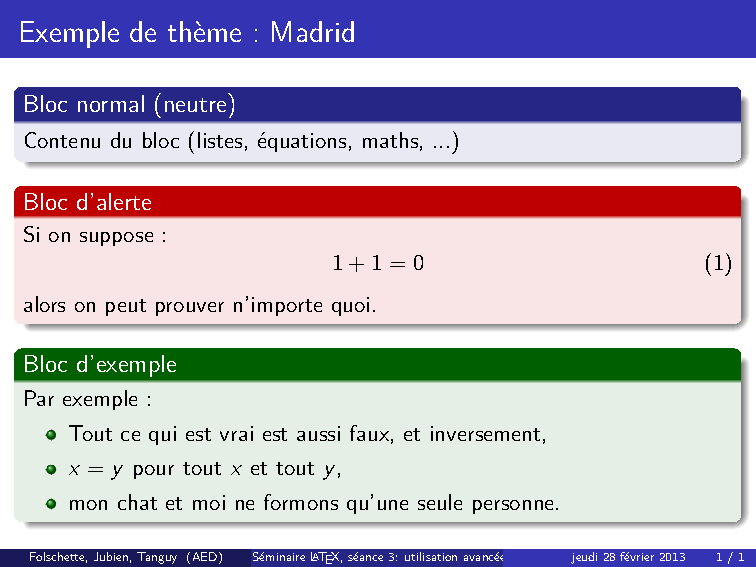
\includegraphics[width=1\textwidth]{ppt_seance3_exblock}
\end{figure}
\end{frame}



\section{Les animations en Beamer}

\begin{frame}[fragile]
  \frametitle{Animations}

On peut définir des animations (statiques) au sein des présentations.
\begin{itemize}
  \item<2,4-> Elles consistent en des apparitions...
  \item<3-> ...ou des disparitions.
\end{itemize}

\bigskip
\pause[4]
Les animations créent plusieurs pages pour la même diapositive, avec les différences nécessaires. La numérotation n'est pas affectée.

\medskip
L'option \lstinline?handout? du \lstinline?\documentclass? permet de supprimer ou de simplifier ces animations.
\end{frame}



\begin{frame}[fragile]
  \frametitle{Apparitions successives}

Avec la commande \lstinline?\pause? ou \lstinline?\pause[x]?

\medskip
Exemple :

\begin{columns}
  \begin{column}{0.20\textwidth}
\begin{lstlisting}
| Texte 1
| \pause
| Texte 2
| 
| \pause
| Texte 3
| \pause
| Texte 4
| \pause[3]
| Texte 5
\end{lstlisting}
  \end{column}
  \begin{column}{0.35\textwidth}
\rmfamily
Texte 1
\pause{}
Texte 2

\pause
Texte 3
\pause{}
Texte 4
\pause[3]
Texte 5
  \end{column}
\end{columns}
\end{frame}



\begin{frame}[fragile]
  \frametitle{Animations avancées}

Deux commandes :
\begin{itemize}
  \item \lstinline?\only<pages>{contenu}? dévoile \lstinline?contenu? uniquement dans les \lstinline?pages? spécifiées,
  \item \lstinline?\uncover<pages>{contenu}? fait de même, mais réserve l'espace non occupé lorsqu'il n'est pas affiché.
\end{itemize}

Le \lstinline?contenu? peut contenir n'importe quoi (texte, figures, mathématiques, etc.).

Les \lstinline?<pages>? sont définies par groupes :
\begin{itemize}
  \item \lstinline?<n>? : la page $n$,
  \item \lstinline?<-n>? : toutes les pages avant $n$ compris,
  \item \lstinline?<n->? : toutes les pages à partir de $n$,
  \item \lstinline?<n-p>? : toutes les pages entre $n$ et $p$ inclus,
  \item \lstinline?<x,y>? : le groupe de pages $x$ et le groupe de pages $y$.
\end{itemize}
\end{frame}



\begin{frame}[fragile]
  \frametitle{Animations avancées}

Exemple avec \lstinline?\only? et \lstinline?\uncover? :
\begin{columns}
  \begin{column}{0.35\textwidth}
\begin{lstlisting}
| Texte 1.
| 
| \uncover<2->{
|   Texte 2 ?
|   \only<2-4>{Texte 3...}
|   \uncover<3>{Texte 4 !}
|   Texte 5.
| }
| \pause[5]
\end{lstlisting}
  \end{column}
  \begin{column}{0.60\textwidth}
\rmfamily
Texte 1.

\uncover<2->{
  Texte 2 ?
  \only<2-4>{Texte 3...}
  \uncover<3>{Texte 4 !}
  Texte 5.
}
\pause[5]
  \end{column}
\end{columns}
\end{frame}



\begin{frame}[fragile]
  \frametitle{Animations avancées}

D'autres commandes peuvent prendre un argument \lstinline?<pages>? optionnel.

\bigskip
Exemple : \lstinline?\item<pages>?
\begin{columns}
  \begin{column}{0.40\textwidth}
\begin{lstlisting}
\begin{itemize}
  \item<1,5> Premier £\'e£l£\'e£ment
  \item<2,4-> Second £\'e£l£\'e£ment
  \item<3-> Troisi£\`e£me £\'e£l£\'e£ment
\end{itemize}\end{lstlisting}
  \end{column}
  \begin{column}{0.40\textwidth}
\rmfamily
\begin{itemize}
  \item<1,5> Premier élément
  \item<2,4-> Second élément
  \item<3-> Troisième élément
\end{itemize}
  \end{column}
\end{columns}

\pause[5]
\end{frame}



\begin{frame}[fragile, t]
  \frametitle{Animations TikZ}

\begin{figure}
  \begin{tikzpicture}
    \tikzexnodes
    \tikzexedges
\node<2> at (rond) [rectangle, fill=green!20, draw, thick] {Oui !} ;
\node<3> at (ellipse) [rectangle, fill=red!20, draw, thick] {Non !} ;
  \end{tikzpicture}
\end{figure}

\bigskip
Beaucoup de commandes TikZ acceptent aussi la syntaxe \lstinline?<pages>? pour créer des animations dans une présentation.

\bigskip
\begin{lstlisting}
\node<2> at (rond) [square, fill=green!20, draw, thick] {Oui !} ;
\node<3> at (ellipse) [square, fill=red!20, draw, thick] {Non !} ;
\end{lstlisting}
\end{frame}



\section{Personnalisation de Beamer}

\begin{frame}[fragile]
  \frametitle{Les thèmes}

Il est possible d'utiliser des thèmes prédéfinis pour modifier l'apparence et les couleurs d'une présentation. On peut spécifier :
\begin{itemize}
  \item Un thème d'agencement avec \lstinline?\usetheme{theme}? :
  \begin{itemize}
    \item style de la page de titre et agencement des diapos,
    \item forme et contenu des bandeaux,
    \item police, forme des puces, ...
  \end{itemize}
  Exemples : \lstinline?Warsaw?, \lstinline?Madrid?, \lstinline?Copenhagen?, \lstinline?CambridgeUS?...
  \item Un thème de couleurs avec \lstinline?\usecolortheme{theme}? :
  \begin{itemize}
    \item couleur du texte, des titres, du sommaire,
    \item couleur de fond, des blocs, des bandeaux...
  \end{itemize}
  Exemples : \lstinline?beaver?, \lstinline?dolphin?, \lstinline?dove?, \lstinline?fly?...
\end{itemize}

\bigskip
Pour une liste des thèmes par défaut, voir le WikiBooks \cite{wikibooksbeamer}.
\end{frame}



\begin{frame}[fragile]
  \frametitle{Personnaliser un thème}

Il est aussi possible de personnaliser en partie un thème ou de créer un thème, pour :
\begin{itemize}
  \item modifier le contenu des bandeaux d'en-tête et de pied,
  \item revoir l'agencement,
  \item supprimer des éléments inutiles (sommaire, icônes...),
  \item adapter certaines couleurs.
\end{itemize}

\bigskip
On peut pour cela redéfinir toutes les caractéristiques d'une présentation :
\begin{itemize}
  \item les agencements,
  \item les couleurs.
\end{itemize}

\bigskip
Pour une liste des options modifiables, voir le WikiBooks \cite{wikibooksbeamer}.
\end{frame}



\begin{frame}[fragile]
  \frametitle{Exemple de thème : CambridgeUS}

\begin{block}{Bloc normal (neutre)}
  Contenu du bloc (listes, équations, maths, ...)
\end{block}

\begin{alertblock}{Bloc d'alerte}
  Si on suppose :
  \begin{equation}
    1+1=0
  \end{equation}
  alors on peut prouver n'importe quoi.
\end{alertblock}

\begin{exampleblock}{Bloc d'exemple}
  Par exemple :
  \begin{itemize}
    \item Tout ce qui est vrai est aussi faux, et inversement,
    \item $x = y$ pour tout $x$ et tout $y$,
    \item mon chat et moi ne formons qu'une seule personne.
  \end{itemize}
\end{exampleblock}
\end{frame}



\begin{frame}[plain]
\begin{figure}
  \centering
  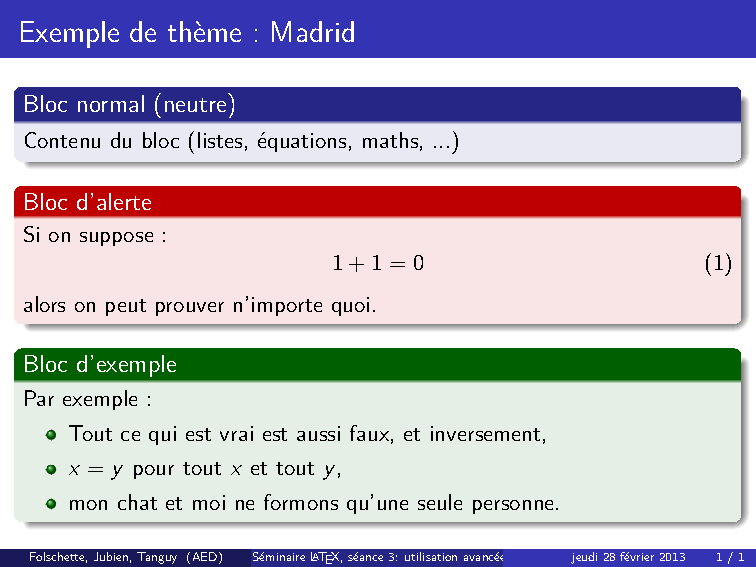
\includegraphics[width=1\textwidth]{ppt_seance3_exblock}
\end{figure}
\end{frame}



\begin{frame}[plain]
\begin{figure}
  \centering
  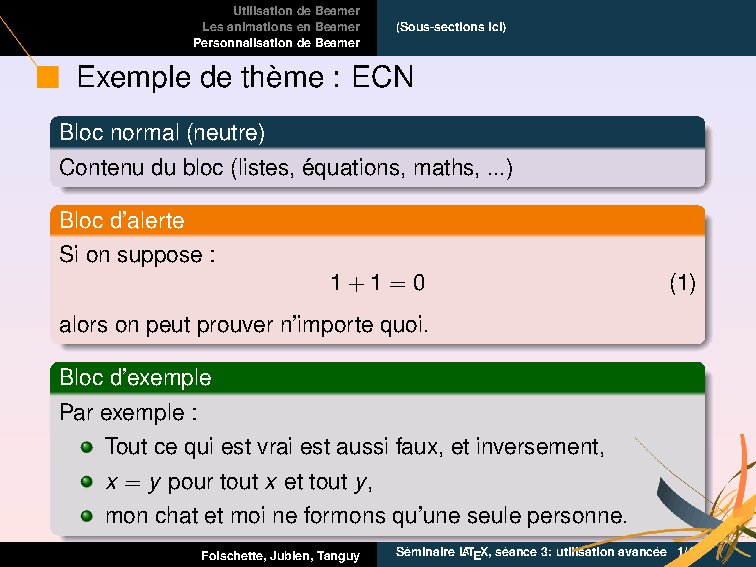
\includegraphics[width=1\textwidth]{ppt_seance3_extheme_ecn}
\end{figure}
\end{frame}



\begin{frame}[fragile]
  \frametitle{Exercice}

Une présentation simple :

\begin{lstlisting}[multicols=2]
  \documentclass{beamer}

  \usepackage[french]{babel}
  \usepackage[utf8]{inputenc}

  \usetheme{Madrid}
  \usecolortheme{default}

  \title{Pr£\'e£sentation de ma th£\`e£se}
  \author{Pr£\'e£nom Nom}
  \institute[LDC]{Laboratoire des Chatons}

  \begin{document}

  \begin{frame}
    \maketitle
  \end{frame}

  
  \section{£\`A£ propos de moi}

  \begin{frame}
    \frametitle{Ce que j'aime}
    \begin{itemize}
      \item Les chatons,
      \pause
      \item le jus de raisin,
      \pause
      \item etc.
    \end{itemize}
  \end{frame}

  \end{document}
\end{lstlisting}

\end{frame}




%%% Bibliographie %%%

\begin{frame}
  \frametitle{Bibliographie}

\nocite{*}
\bibliographystyle{abbrv-fr}
\bibliography{latex}
\end{frame}


%%%%%%%%%%%%%%%%%%%%%%%%%%%%%%%%%%%%%%%%%%%%%%%%%%%%%%%%%%%%%%%%%%%%%%%%%%%%%%%%%%
%%%%%%%%%%%%%%%%%%%%%%%% FIN DU DOCUMENT %%%%%%%%%%%%%%%%%%%%%%%%%%%%%%%%%%%%%%%%%%%%%%%%
%%%%%%%%%%%%%%%%%%% ( NON PRISE EN COMPTE DE LA SUITE ) %%%%%%%%%%%%%%%%%%%%%%%%%%%%%%%%%%%%%%%%%%%
\end{document}
%%%%%%%%%%%%%%%%%%%%%%%%%%%%%%%%%%%%%%%%%%%%%%%%%%%%%%%%%%%%%%%%%%%%%%%%%%%%%%%%%%
%%%%%%%%%%%%%%%%%%%%%%%%%%%%%%%%%%%%%%%%%%%%%%%%%%%%%%%%%%%%%%%%%%%%%%%%%%%%%%%%%%
